\documentclass[10pt,twocolumn,letterpaper]{article}
\usepackage[review,applications]{wacv}
\usepackage{amsmath,amssymb,booktabs,multirow}
\usepackage{graphicx}
\usepackage{microtype}
\usepackage{xcolor}
\usepackage{enumitem}
\usepackage{mathtools}
\usepackage{algorithm}
\usepackage{algpseudocode}
\usepackage{array}
\usepackage{tabularx}

\newcommand{\OrnaScout}{\textsc{OrnaScout}}
\newcommand{\Tset}{\mathcal{T}}
\newcommand{\Eset}{\mathcal{E}}
\newcommand{\R}{\mathbb{R}}
\newcommand{\yes}{\textsc{yes}}
\newcommand{\no}{\textsc{no}}
\setlist[itemize]{leftmargin=*,nosep}
\setlist[enumerate]{leftmargin=*,nosep}

\newcolumntype{Y}{>{\raggedright\arraybackslash}X}
\newcolumntype{C}[1]{>{\centering\arraybackslash}p{#1}}

\definecolor{wacvblue}{rgb}{0.21,0.49,0.74}
\usepackage[pagebackref,breaklinks,colorlinks,allcolors=wacvblue]{hyperref}

\def\wacvPaperID{2841}
\def\confName{WACV}
\def\confYear{2027}

\title{OrnaScout: Supplementary Material}
\author{Anonymous WACV submission}

\begin{document}
\maketitle

\section{Scope and Evidence Boundary}

This supplement makes the source-safe construction, budgeted evidence
selection, structured prediction, and selective evaluation auditable.  Only
the frozen corpus audit and validation selector study support quantitative
claims.  Model and risk-gate definitions specify the common protocol; smoke
tests and incomplete runs are not experimental results.

\paragraph{Claim boundary.}
The two-crop dataset is not a universal nursery benchmark.  The detector
supplies evidence candidates, not plant-health diagnoses; the VLM emits a
scouting record, not an agronomic recommendation.  Selector choices use
validation sources only.  Oracle routing and shuffled scores are diagnostic
controls, not deployable methods.

\section{Corpus Audit and Cross-Crop Shift}
\label{sec:data}

The source corpus contains 418 high-resolution UAV RGB images: 297 Magnolia
and 121 Azalea.  Magnolia frames are $5184\!\times\!3888$ pixels and Azalea
frames are $5280\!\times\!3956$ pixels.  We retain 29,842 valid one-class plant
boxes (15,644 Magnolia; 14,198 Azalea).  Five zero-width rows are rejected by
the parser without modifying the source labels.  Three empty Azalea label
files are retained as source-level negatives, while one unmatched RGB image is
excluded.  No box extends outside its source frame, and the duplicate-image
audit finds no candidate duplicate pair.  \Cref{tab:corpus} summarizes the
frozen source, annotation, split, and tile counts.

\begin{table}[t]
\centering
\caption{Frozen corpus and source-safe split.  Tile counts include positive
and hard-negative tiles generated after the source-image split.}
\label{tab:corpus}
\small
\setlength{\tabcolsep}{3.5pt}
\begin{tabular}{lrrrr}
\toprule
Crop & Sources & Boxes & Train/Val/Test & Tiles \\
\midrule
Azalea   & 121 & 14,198 & 81/20/20  & 4,235 \\
Magnolia & 297 & 15,644 & 221/38/38 & 10,395 \\
\midrule
Total    & 418 & 29,842 & 302/58/58 & 14,630 \\
\bottomrule
\end{tabular}
\end{table}

The two crops impose a meaningful visual shift.  Azalea sources contain a
median of 97 boxes, compared with 57 for Magnolia, while the median normalized
Azalea box area is $0.00466$, 44.1\% smaller than Magnolia's $0.00833$.
Median brightness is similar (0.400 versus 0.395), but the green-pixel fraction
is lower for Azalea (0.312 versus 0.429).  These differences jointly change
object scale, density, texture, and background composition; they motivate
bidirectional transfer rather than a pooled-only report.
\begin{figure*}[t]
\centering
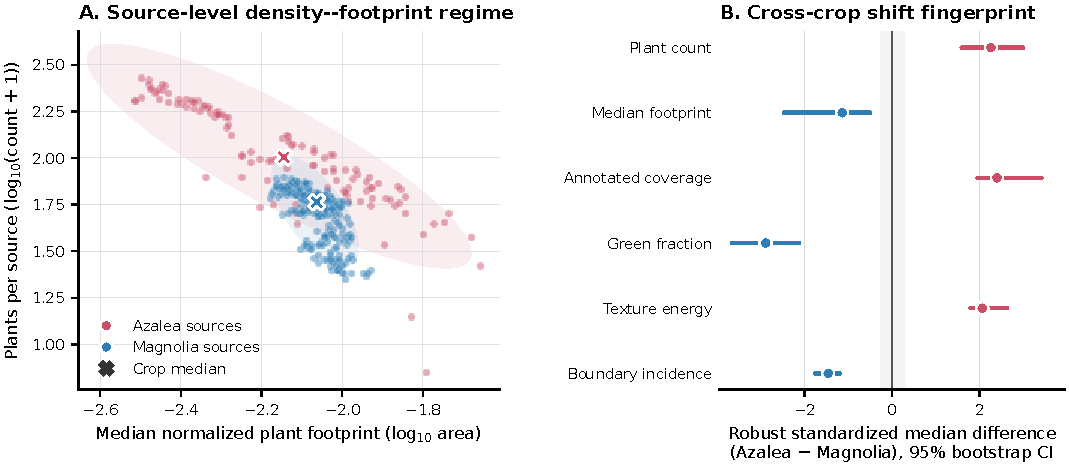
\includegraphics[width=.98\textwidth]{figures/cross_crop_signature.pdf}
\caption{Source-level cross-crop shift.  \textbf{A:} Each point is one source
image; crosses and ellipses show crop medians and 90\% covariance regions in
the density--footprint plane.  \textbf{B:} Robust standardized Azalea-minus-
Magnolia median differences with 95\% source-bootstrap confidence intervals
(1,000 resamples).  Positive values indicate larger Azalea statistics.  The
joint reversal in plant density, footprint, green fraction, and texture makes
cross-crop transfer a multivariate shift rather than a class-count imbalance.}
\label{fig:cross-crop-signature}
\end{figure*}

Across both crops, 28.96\% of boxes are close to a source-image boundary.
This is relevant because overlapping crops can preserve a box in more than one
tile; consequently, tile-level random splitting would leak near-identical
content across partitions.  We therefore use source identity as the indivisible
unit for splitting, resampling, and uncertainty estimation.
\Cref{fig:cross-crop-signature} visualizes this source-level shift without
treating correlated tiles as independent observations.

\section{Source-Safe Preparation}
\label{sec:preparation}

\paragraph{Split before tiling.}
Each source image is assigned to train, validation, or test before any crop is
written.  All tiles and labels derived from one source inherit that assignment.
The frozen seed is 2026.  The resulting split contains 302/58/58 source images
and 10,570/2,030/2,030 tiles for train/validation/test.  The split is stratified
by crop and source-level annotation density; sibling tiles cannot cross
partitions.

\paragraph{Overlapping tiling.}
Images are tiled at $1024\!\times\!1024$ pixels with 25\% overlap.  For a source
box $b$ and tile $t$, let
\begin{equation}
v(b,t)=\frac{\operatorname{area}(b\cap t)}{\operatorname{area}(b)}.
\label{eq:visible}
\end{equation}
The clipped box is assigned to $t$ when $v(b,t)\geq0.5$.  This rule retains
partially visible plants while preventing small box fragments from becoming
positive labels.  A retained box is marked boundary-truncated when its maximum
visible fraction lies in $[0.5,0.98)$.  Empty tiles from labeled source images
form the hard-negative set; 1,328 such tiles are present after preparation.

\paragraph{Derived tasks.}
For each tile, the annotation count induces the bins
\(\{0,1\text{--}5,6\text{--}15,16\text{--}30,{>}30\}\).
Density belongs to \{empty, sparse, moderate, dense\}; coverage belongs to
\{none, low, medium, high\}.  These labels are generated deterministically from
the separate ground-truth file.  They are never embedded in the inference
manifest or prompt.  \Cref{alg:prepare} gives the complete preparation and
separation procedure.

\begin{algorithm}[t]
\caption{Source-safe preparation}
\label{alg:prepare}
\begin{algorithmic}[1]
\Require source images $\mathcal{I}$, labels $\mathcal{B}$, tile size $s$,
overlap $o$, visible threshold $\tau$
\Ensure inference manifest $\mathcal{M}$ and disjoint ground truth $\mathcal{G}$
\State validate image--label pairs and reject malformed boxes
\State assign each source $I$ to train, validation, or test
\For{each source image $I$}
  \State generate overlapping windows of size $s$ and stride $s(1-o)$
  \For{each window $t$}
    \State clip boxes to $t$ and retain those with $v(b,t)\geq\tau$
    \State write RGB tile and inference prompt to $\mathcal{M}$
    \State write task labels and provenance only to $\mathcal{G}$
  \EndFor
\EndFor
\State assert that no source ID occurs in more than one split
\end{algorithmic}
\end{algorithm}

\section{Budgeted Evidence Selection}
\label{sec:selector}

Let $\Tset(I)=\{t_i\}_{i=1}^{N_I}$ be the tiles from source image $I$.
The detector produces confidence $c_i\in[0,1]$ and predicted count $n_i$.
The evidence score is
\begin{equation}
q_i=c_i+\frac{\min(n_i,20)}{20}.
\label{eq:score}
\end{equation}
The cap prevents a single unusually dense tile from dominating the ranking.
For budget $K$ and exploration ratio $\rho$, we set
\begin{equation}
K_{\mathrm{explore}}=\operatorname{round}(\rho K),\qquad
K_{\mathrm{exploit}}=K-K_{\mathrm{explore}}.
\label{eq:allocation}
\end{equation}
The selected set is
\begin{equation}
\Eset_K(I)=
\operatorname{TopK}_{K_{\mathrm{exploit}}}(q_i)
\cup
\operatorname{Explore}_{K_{\mathrm{explore}}}
(\Tset(I)\setminus\Eset_{\mathrm{exploit}}).
\label{eq:selector}
\end{equation}
The default $K=8$, $\rho=0.25$ therefore uses six exploitative and two
exploratory tiles.  All VLMs receive exactly the same selected images and task
schema for a given source.

\paragraph{Validation metrics.}
For source objects $\mathcal{B}_I$, evidence recall at threshold $\eta=0.5$ is
\begin{equation}
R_{\mathrm{ev}}(I)=\frac{1}{|\mathcal{B}_I|}
\sum_{b\in\mathcal{B}_I}
\mathbf{1}\!\left[\max_{t\in\Eset_K(I)}v(b,t)\geq\eta\right].
\label{eq:evidence-recall}
\end{equation}
Spatial coverage is the union area of selected tiles divided by source area.
Overlap redundancy is
\begin{equation}
D_{\mathrm{ov}}(I)=
\frac{\sum_{t\in\Eset_K(I)}\operatorname{area}(t)}
{\operatorname{area}(\cup_{t\in\Eset_K(I)}t)}-1.
\label{eq:redundancy}
\end{equation}
We additionally report boundary-truncation rate and the fraction of prepared
hard-negative tiles retained by a selector.  Confidence intervals use 1,000
source-level bootstrap resamples.  Randomized selectors use ten repetitions.
\Cref{tab:selector-b8} reports the matched $K=8$ comparison.

\begin{table*}[t]
\centering
\caption{Validation-only selector audit at $K=8$.  Values are source means;
parentheses give source-bootstrap 95\% confidence intervals.  Oracle and
shuffled-score controls are omitted because they are diagnostics, not
deployable selectors.}
\label{tab:selector-b8}
\small
\setlength{\tabcolsep}{4.5pt}
\begin{tabular}{lccccc}
\toprule
Selector & Evidence recall & Spatial coverage & Redundancy & Boundary trunc. & Hard-neg. recall \\
\midrule
Random & .352 (.335--.382) & .361 (.359--.364) & .141 (.136--.146) & .459 (.423--.492) & .231 (.209--.253) \\
Spatial uniform & .438 (.415--.464) & .411 (.409--.413) & .000 (.000--.000) & .401 (.371--.431) & .196 (.136--.257) \\
Confidence top-$K$ & .384 (.350--.425) & .340 (.334--.346) & .214 (.194--.234) & .495 (.449--.538) & .024 (.000--.065) \\
Count top-$K$ & \textbf{.455} (.420--.496) & .330 (.324--.337) & .252 (.226--.282) & \textbf{.398} (.359--.437) & .015 (.000--.043) \\
Combined top-$K$ & .451 (.416--.494) & .330 (.324--.336) & .254 (.229--.285) & .474 (.424--.516) & .007 (.000--.018) \\
Exploit--explore & .439 (.410--.474) & .345 (.341--.349) & .196 (.183--.212) & .486 (.438--.529) & .067 (.050--.085) \\
\bottomrule
\end{tabular}
\end{table*}

The audit exposes a genuine trade-off rather than a uniformly dominant method.
Count top-$K$ yields the highest validation evidence recall at $K=8$.
Exploit--explore reduces overlap redundancy by 22.7\% relative to combined
top-$K$ and raises hard-negative retention from 0.7\% to 6.7\%, but its evidence
recall is lower by 1.2 points.  The operating point must therefore match the
downstream reliability objective rather than maximize one metric alone.

\begin{figure*}[t]
\centering
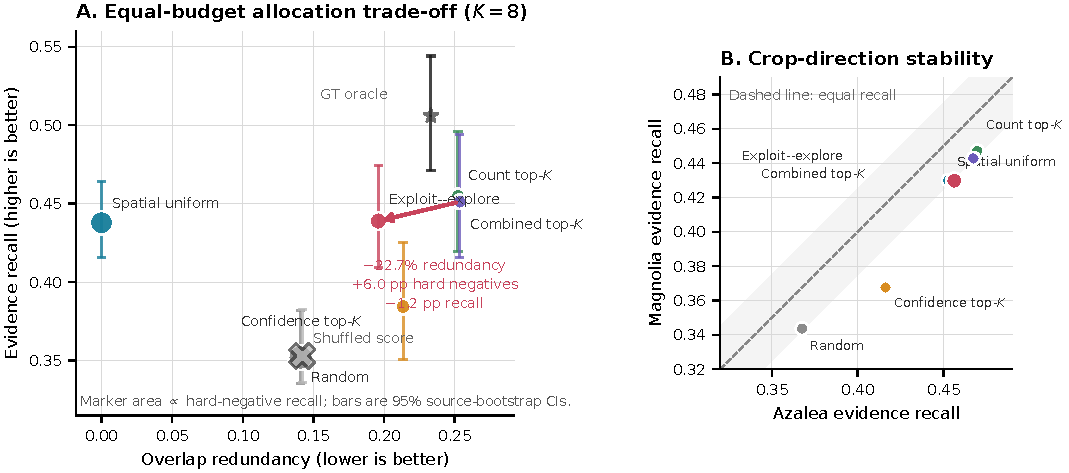
\includegraphics[width=.98\textwidth]{figures/selector_tradeoff_map.pdf}
\caption{Mechanism-level selector audit at the matched budget $K=8$.
\textbf{A:} Evidence recall versus overlap redundancy; vertical bars are 95\%
source-bootstrap intervals and marker area is proportional to hard-negative
recall.  Stars denote non-deployable diagnostics.  The arrow isolates the
combined-to-exploit--explore change.  \textbf{B:} Crop-specific evidence recall;
distance from the equality line reveals directional sensitivity that a pooled
mean would hide.}
\label{fig:selector-tradeoff}
\end{figure*}

\Cref{fig:selector-tradeoff} exposes the equal-budget trade-off and crop
direction, while \cref{fig:selector-sweep} tests whether it persists across the
complete budget range.

\begin{figure*}[t]
\centering
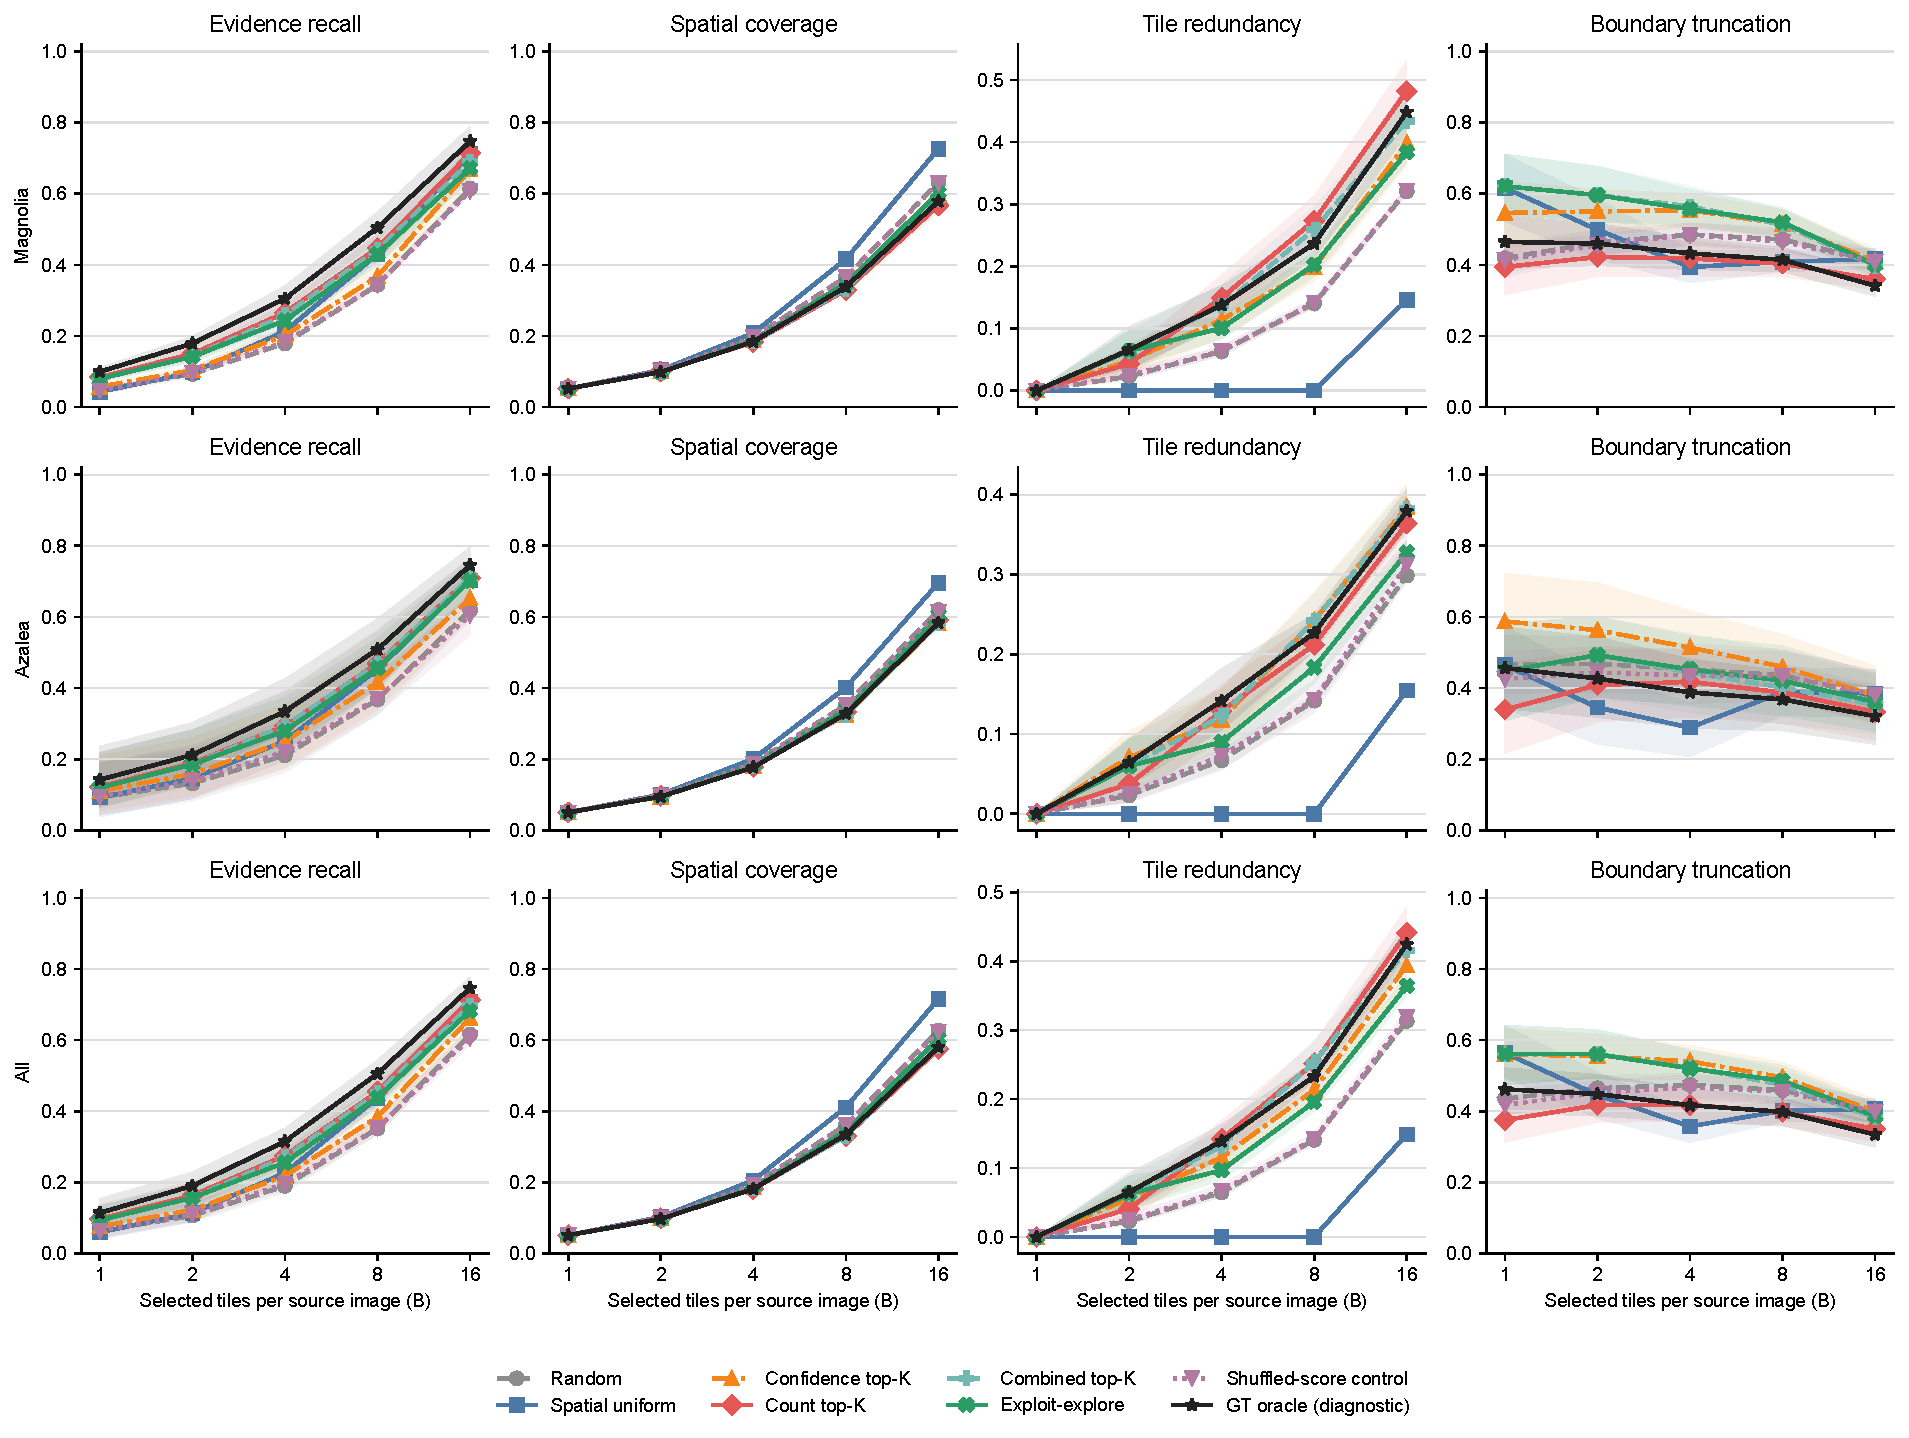
\includegraphics[width=.98\textwidth]{figures/selector_budget_audit.pdf}
\caption{Complete validation-only budget sweep.  Curves show source-level
means and 95\% source-bootstrap intervals across both crop domains and their
pooled source set.}
\label{fig:selector-sweep}
\end{figure*}

\section{Prompt, Schema, and Model Interface}
\label{sec:schema}

\paragraph{Frozen tile prompt.}
The following instruction is supplied with each selected RGB tile:
\begin{quote}\small
Inspect this UAV RGB nursery tile. Return one JSON object using exactly the
nine fields in \cref{tab:schema}. Use only the listed categories and a
confidence in $[0,1]$. Describe visible evidence only; use unknown and request
human review when evidence is insufficient.
\end{quote}
The inference manifest contains image paths, prompts, split, and anonymous
provenance identifiers.  Ground-truth labels reside in a separate file and are
joined only during evaluation.

\paragraph{Schema validation.}
The parser extracts the first JSON object, checks all required keys, enforces
categorical vocabularies, and validates numeric confidence.  Malformed output
is retained as a failure; it is never silently repaired into a valid record.
The nine-field schema is summarized in Table~\ref{tab:schema}.

\begin{table}[t]
\centering
\caption{Structured output schema.}
\label{tab:schema}
\small
\begin{tabularx}{\columnwidth}{lY}
\toprule
Field & Valid values or interpretation \\
\midrule
crop type & azalea, magnolia, unknown \\
presence & yes, no \\
count bin & 0; 1--5; 6--15; 16--30; $>$30 \\
density & empty, sparse, moderate, dense \\
coverage & none, low, medium, high \\
visual evidence & concise visible-evidence text \\
priority & low, medium, high \\
confidence & scalar in $[0,1]$ \\
human review & yes, no \\
\bottomrule
\end{tabularx}
\end{table}

\paragraph{Model families.}
Four public VLM configurations are registered: SmolVLM2-500M and
SmolVLM2-2.2B~\cite{huggingface2025smolvlm2}, Phi-3.5-Vision
\cite{microsoft2024phi35vision}, and LLaVA-1.5-7B~\cite{liu2024llava15}.
The registry freezes the corresponding Hugging Face model-card IDs and the
Phi revision hash.  Zero-shot and adapted models are reported separately; a
compatibility smoke test is not an evaluation result.

\section{Reliability and Evaluation Protocol}
\label{sec:eval}

\paragraph{Task metrics.}
We report macro-F1 for crop type, presence, count bin, density, and coverage,
plus exact schema validity.  A task macro-F1 averages the five task-level
macro-F1 values so that a dense count category cannot dominate the report.
All intervals and paired differences cluster by source image.  Tile-level
confidence intervals are not used because overlapping tiles are correlated.

\paragraph{Repeat consistency.}
For repeated generations $\{\hat y^{(r)}\}_{r=1}^{R}$ and categorical task set
$\mathcal{K}$, consistency is the mean modal agreement
\begin{equation}
C=\frac{1}{|\mathcal{K}|}\sum_{k\in\mathcal{K}}
\frac{1}{R}\max_{a}\sum_{r=1}^{R}\mathbf{1}[\hat y_k^{(r)}=a].
\label{eq:consistency}
\end{equation}
The final experiment uses three generations under identical decoding settings.

\paragraph{Risk score and abstention.}
The fixed diagnostic score combines schema validity $s$, repeat consistency
$C$, VLM confidence $p$, and detector agreement $d$:
\begin{equation}
u_{\mathrm{fixed}}=.35s+.25C+.20p+.20d.
\label{eq:fixed-gate}
\end{equation}
The proposed gate is a validation-fitted failure predictor using the same
signals.  Its threshold is selected on validation data and frozen before test
evaluation.  We report risk--coverage curves, area under the risk--coverage
curve (AURC), accepted risk, false-accept rate, and coverage.  Verified empty
sources define the hallucination denominator; ordinary detector misses do not
automatically become VLM hallucinations.

\paragraph{Cross-crop protocols.}
The complete matrix contains Magnolia$\rightarrow$Magnolia,
Azalea$\rightarrow$Azalea, Magnolia$\rightarrow$Azalea,
Azalea$\rightarrow$Magnolia, and pooled training/testing.  Model selection,
selector choice, risk threshold, and prompt are frozen on training/validation
sources for each protocol.  No test source contributes to threshold fitting.

\paragraph{Efficiency.}
Latency excludes download and reports model loading separately.  Runs record
warm-up, batch size, precision, generation limit, hardware, and peak incremental
memory.  Matched comparisons use the same budget and prompt; all-tile inference
is an efficiency baseline, not a matched-input accuracy baseline.

\section{Controlled Ablation Matrix}
\label{sec:ablation}

The ablation design changes one factor at a time while preserving source
splits, ground truth, prompt, generation limit, and source-level bootstrap
protocol.  Table~\ref{tab:ablations} distinguishes the measured selector
evidence analysis from model-dependent evaluation components.  Only the former
is used for quantitative claims in this supplement.

\begin{table*}[t]
\centering
\caption{Controlled factors and their scientific questions.  ``Measured''
denotes the frozen validation evidence audit; ``protocol'' denotes an
evaluation definition without a quantitative claim in this supplement.}
\label{tab:ablations}
\small
\begin{tabularx}{.98\textwidth}{lYYl}
\toprule
Factor & Compared settings & Primary response & Evidence status \\
\midrule
Selection rule & random, spatial, confidence, count, combined, exploit--explore
& evidence recall, coverage, redundancy, hard-negative recall & measured \\
Visual budget & $K\in\{1,2,4,8,16\}$
& task F1 versus latency/memory and evidence recall & measured routing \\
Exploration & $\rho\in\{0,.10,.25,.50\}$
& recall--redundancy--negative-retention trade-off & measured routing \\
Tile geometry & size and overlap sweep
& boundary truncation, task F1, source cost & protocol \\
Gate signals & schema; +consistency; +detector; fitted gate
& AURC, false accepts, accepted risk, coverage & protocol \\
Generation repeats & one versus three
& consistency, latency, accepted risk & protocol \\
Model capacity & 500M, 2.2B, Phi-3.5-V, LLaVA-7B
& matched-budget task F1, schema validity, memory & protocol \\
Cross-crop direction & M$\rightarrow$A, A$\rightarrow$M, within-crop, pooled
& transfer gap and failure composition & protocol \\
\bottomrule
\end{tabularx}
\end{table*}

\paragraph{Paired reporting.}
Selector comparisons are paired by source image.  For each bootstrap resample,
we sample source IDs with replacement, retain all associated tiles, and compute
the difference between methods.  This directly estimates whether a routing
change helps the same aerial scenes.  Mean$\pm$standard-deviation over tiles is
not used as a substitute for source-clustered uncertainty.

\paragraph{Operating-point discipline.}
The full sweep accompanies the single validation-selected operating point and
its trade-off curve.  No operating point is changed after inspecting the test
set.  Because the chosen selector is not best on every validation metric, it is
interpreted through the stated recall, redundancy, and negative-retention
trade-off rather than as uniformly dominant.

\section{Annotation Review and Failure Taxonomy}
\label{sec:audit}

The automatic label audit checks pairing, normalized coordinates, zero-area
boxes, frame excursions, empty labels, annotation density, normalized box
area, and possible image duplication.  It does not prove semantic correctness.
A separate review sheet therefore samples boxes across crop, source, box-size
stratum, image boundary, and annotation-density stratum.  Reviewers mark
correct, loose, tight, duplicate, wrong-object, or ambiguous.  Because the
frozen artifacts do not contain adjudicated review sheets, this supplement
makes no semantic annotation-acceptance claim.  This distinction prevents an
automated format audit from being misreported as human semantic validation.

\paragraph{Failure taxonomy.}
Qualitative analysis uses balanced denominators.  Detector failures comprise
misses, background false positives, duplicates, and boundary truncation; VLM
failures comprise task errors, malformed schema, unsupported claims, and repeat
inconsistency.  Gate outcomes distinguish correct/false acceptance from
correct/unnecessary abstention.  Displayed cases identify crop, protocol,
ground truth, prediction, selector, budget, and gate decision.

Hard-negative mining may be evaluated as a detector-training ablation only
when the mined negatives, held-out split, and before/after checkpoints are
available under the same source-safe protocol.  Results from a separate
pipeline or a screenshot are not merged into the reported experiment.

\section{Reproducibility Checklist}
\label{sec:repro}

The anonymous release record comprises source manifests and hashes; annotation
and rejected-row audits; separate tile, ground-truth, and inference manifests;
the exact prompt, schema, model revisions, and decoding settings; selector
parameters, seeds, and per-source selections; complete prediction JSONL files,
including failures; source-level metrics and bootstrap seeds; gate thresholds;
hardware and efficiency logs; and the scripts generating every table and
figure.

\paragraph{Minimum commands.}
The data preparation and validation selector audit can be reproduced through
the repository entry point:
\begin{verbatim}
python wacv_pipeline.py inspect
python wacv_pipeline.py prepare
python wacv_pipeline.py eda
python wacv_pipeline.py selector-audit \
  --scope combined --split val
\end{verbatim}
Full VLM commands specify model, split, selector, budget, exploration, repeat
count, device, and generation limit.  Test evaluation is separated from
validation-based selector and threshold selection.

\paragraph{Submission audit.}
This review supplement contains no author names, institutional paths, account
identifiers, acknowledgments, or public repository links.  It contains only
material derived from the submitted method and frozen experiments and does not
introduce a post-deadline method change or new dataset.


{\small
\bibliographystyle{ieeenat_fullname}
\bibliography{references}
}

\end{document}
